
% VYSOKOŠKOLSKÁ KVALIFIKAČNÍ PRÁCE
% autor: Michal Struna
% název: Umělá inteligence pro detekci exoplanet z dat pořízených tranzitní metodou
% kódování zdroje: UTF-8

\documentclass[a4paper,12pt]{article}

\usepackage{vskpupa}
\usepackage{listings}
\renewcommand{\lstlistingname}{Zdrojový kód}
\renewcommand{\lstlistlistingname}{Seznam zdrojových kódů}

\expandafter\def\expandafter\UrlBreaks\expandafter{\UrlBreaks%  save the current one
  \do\-}

\let\oldlstlistoflistings\lstlistoflistings
\renewcommand{\lstlistoflistings}{%
  \begingroup%
  \let\oldnumberline\numberline%
  \renewcommand{\numberline}{\lstlistingname~\oldnumberline}%
  \oldlstlistoflistings%
  \endgroup}

\usepackage{color}
\definecolor{lightgray}{rgb}{.9,.9,.9}
\definecolor{darkgray}{rgb}{.4,.4,.4}
\definecolor{gray}{rgb}{0.6, 0.6, 0.6}

\titleformat{\section}
	{\Large\bfseries}
	{\thesection}
	{1em}
	{\MakeUppercase}		% titulky sekcí verzálkami
\titleformat*{\subsection}{\large\rmfamily\bfseries}
\titleformat*{\subsubsection}{\normalsize\rmfamily\bfseries}

% ÚDAJE O PRÁCI
\def\jmenoFakulty{Fakulta elektrotechniky a informatiky}
\def\jmenoAutora{Michal Struna}
\def\nazevPrace{Umělá inteligence pro detekci exoplanet z~dat pořízených tranzitní metodou}
\def\typPrace{Diplomová práce}
\def\rok{2021}
\def\prefixZadani{img/zadani}	% cesta a začátek jména, bude doplněno číslo strany
\def\suffixZadani{.jpg}		% doplní se ke každému jménu souboru zadání
\def\datumOdevzdaniPrace{9.\,5.\,2021}

\long\def\textPodekovani{...}


\long\def\anotace{
...
}
\def\klicovaSlova{exoplanety, extrasolární planety, kepler, umělá inteligence, python}
\def\title{Artificial intelligence for exoplanet detection from transit data}
\long\def\annotation{
...
}
\def\keywords{exoplanet, extrasolar planets, kepler, artificial intelligence, python}

\hypersetup{hidelinks} % Odkazy bez rámečků

%%%%%%%%%%%%%%%%%%%%%%%%%%%%%%%%%%%%%%%%%%%%%%%%%%%%%%%%%%%%
% ZAČÁTEK DOKUMENTU
%%%%%%%%%%%%%%%%%%%%%%%%%%%%%%%%%%%%%%%%%%%%%%%%%%%%%%%%%%%%

\begin{document}

%%%%%%%%%%%%%%%%%%%%%%%%%%%%%%%%%%%%%%%%%%%%%%%%%%%%%%%%%%%%
% ÚVODNÍ STRANY
%%%%%%%%%%%%%%%%%%%%%%%%%%%%%%%%%%%%%%%%%%%%%%%%%%%%%%%%%%%%

\desky
\titulniStrana
\generujZadani
\generujProhlaseni
\podekovaniDolu
\generujPodekovani
\generujAnotaci	
\generujAnnotation
\generujObsah
\generujSeznamObrazku
\lstlistoflistings
\seznamZkratek

\begin{description}[font=\mdseries,leftmargin=6em,labelwidth=!,]
\item[ly]		Light year~--~vzdálenost, kterou světlo ve vakuu urazí za rok
\item[AU]		Astronomical unit~--~Vzdálenost Země od Slunce (149 597 870 km)
\end{description}

%%%%%%%%%%%%%%%%%%%%%%%%%%%%%%%%%%%%%%%%%%%%%%%%%%%%%%%%%%%%
% ÚVOD
%%%%%%%%%%%%%%%%%%%%%%%%%%%%%%%%%%%%%%%%%%%%%%%%%%%%%%%%%%%%

\clearpage
\pagestyle{plain}

\section{Metody hledání exoplanet}

Exoplanety není možné pozorovat přímo vizuálně, protože neemitují žádné světlo a~nachází se ve velkých vzdálenostech od Země. Lze ovšem pozorovat jejich působení na blízké hvězdy nebo jiné útvary, jež jsou pro nás viditelné. K~tomuto účelu se používá několik metod popsaných v této kapitole.

Zdaleka nejvýznamnější je tranzitní metoda, kterou byla objevena většina exoplanet. Velké množství planet bylo objeveno taktéž metodou radiálních vzdáleností. Pomocí ní byly objevovány planety především blízko Země.

\begin{figure}[!htb]
\begin{center}
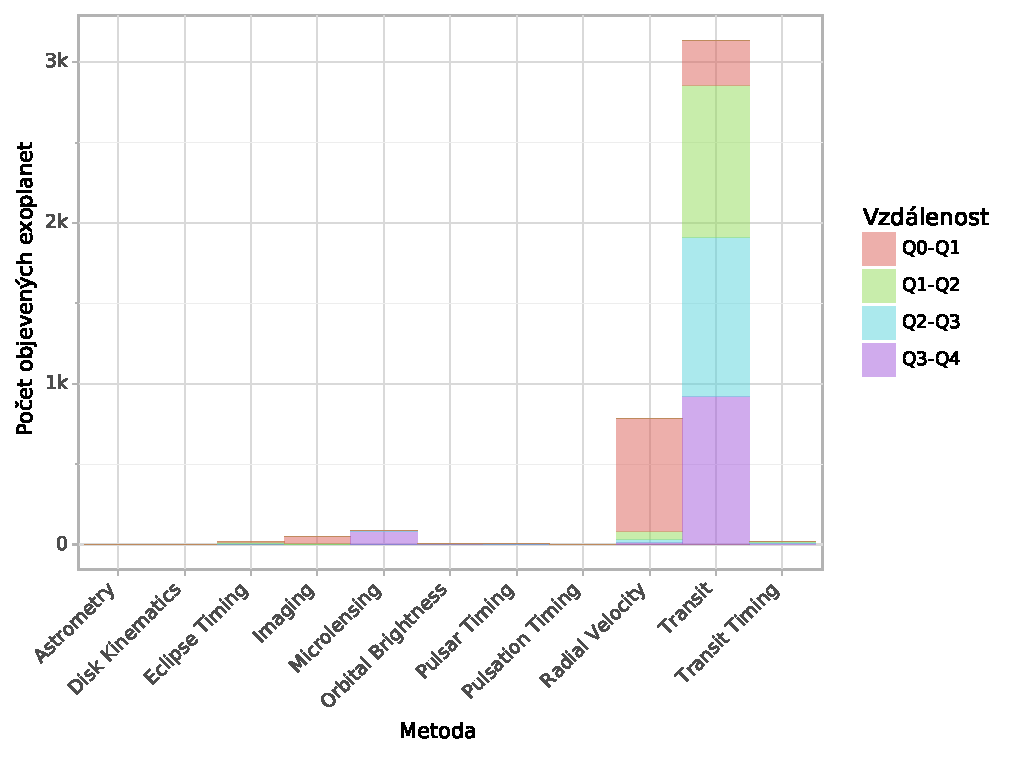
\includegraphics[width=\textwidth]{stats/count_by_method.pdf}
\caption[Vlastnosti planet v závislosti na metodě objevení]{Vlastnosti planet v závislosti na metodě objevení}
\end{center}
\end{figure}

Málo hmotné planety byly objevovány jak tranzitní metodou, tak i~metodou radiálních rychlostí. Naproti tomu hmotné planety blízko své hvězdy byly objeveny především tranzitní metodou, kdežto hmotné planety daleko od své hvězdy metodou radiálních rychlostí. Nejvzdálenější planety od hvězdy byly pak objevovány metodou přímého zobrazení.

\begin{figure}[!htb]
\begin{center}
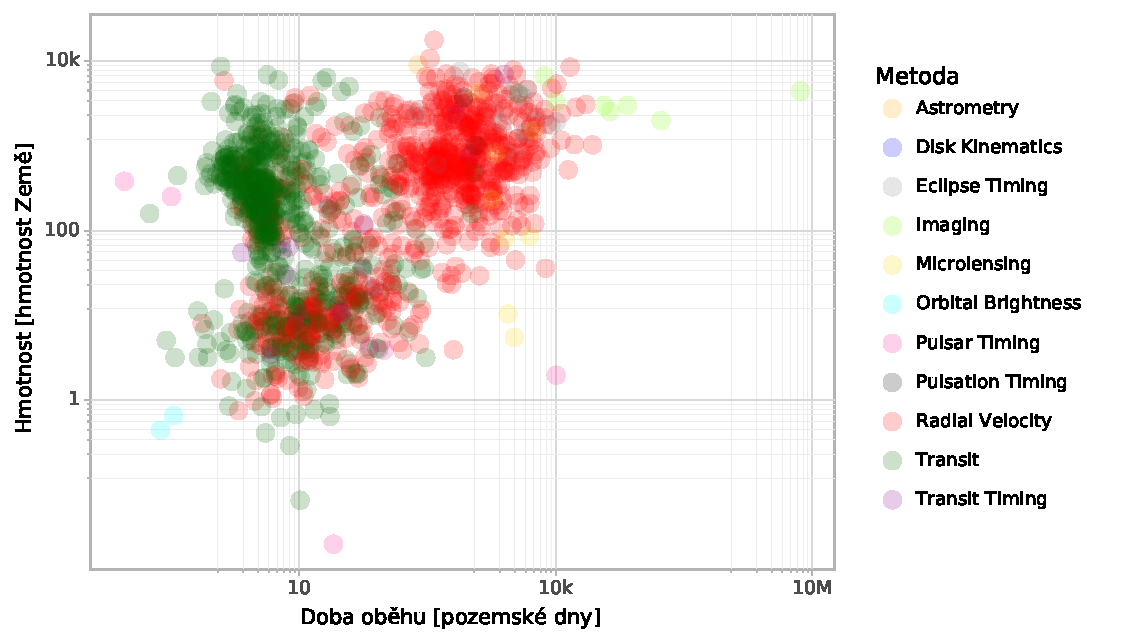
\includegraphics[width=\textwidth]{stats/period_by_mass_by_method.pdf}
\caption[Závislost hmotnosti, periody oběhu a metody objevení planety]{Závislost hmotnosti, periody oběhu a metody objevení planety}
\end{center}
\end{figure}

\clearpage

\subsection{Tranzitní metoda}

Někdy se může exoplaneta při obíhání dostat mezi svou hvězdu a~Zemi. Tento jev se pro pozorovatele na Zemi projeví jako mírný pokles jasu této hvězdy. Pokud je hvězda teleskopem sledována dlouhodobě, je možné v~těchto změnách jasu hvězdy odhalit opakující se složku. To by mohlo indikovat přítomnost nějakého tělesa v~blízkosti této hvězdy.

Tyto změny však nemusí být vždy pravidelné, stejně velké a~na první pohled viditelné. V~systému hvězdy může být více planet, které hvězdu ovlivňují v~různých periodických intervalech, nebo jasnost hvězdy mohou ovlivňovat i~jiné jevy, než obíhající tělesa.

\begin{figure}[!htb]
\begin{center}
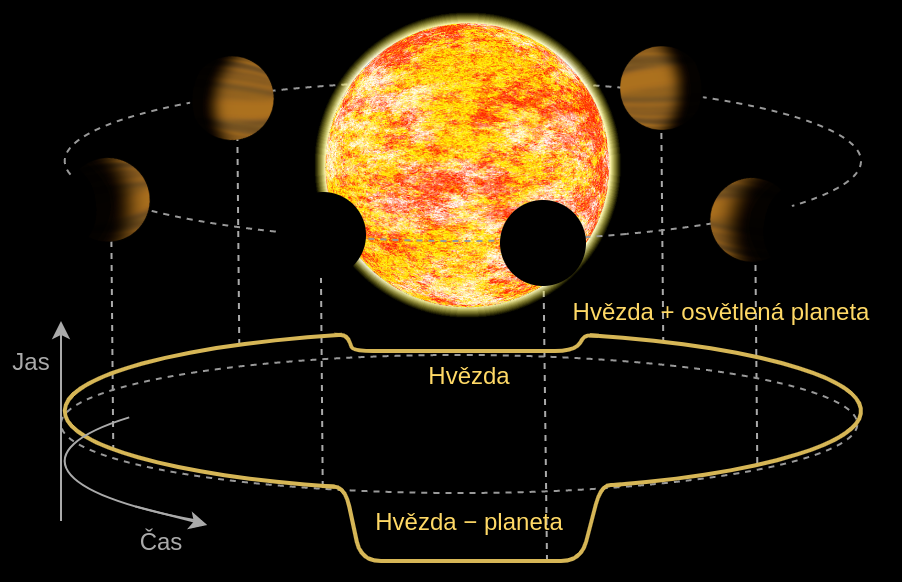
\includegraphics[width=\textwidth]{img/transit.png}
\caption[Tranzitní metoda]{Tranzitní metoda \footnotemark[1]}
\end{center}
\end{figure}

\footnotetext[1]{Vytvořeno autorem v \url{https://www.draw.io} a GIMP.}

Tranzitní metoda vzbuzuje velký zájem především kvůli možnosti objevovat i~malé planety podobné Zemi~--~takové planety by mohly spíše splňovat podmínky pro život. Úspěšnost této metody však silně závisí na geometrii přechodu planety přes hvězdu a~poklesu jasu hvězdy.


\clearpage

\subsection{Metoda radiálních rychlostí}

Stejně jako hvězda ovlivňuje obíhající planetu, tak i~planeta gravitačně ovlivňuje svou hvězdu a~obě tělesa obíhají kolem společného těžiště. Tento pohyb se může projevit jako opakované přibližování a~vzdálování hvězdy vůči pozorovateli na Zemi.

Pokud se zdroj elektromagnetického vlnění (hvězda) přibližuje vůči pozorovateli, vlnění má kratší vlnovou délku a~jeví se více do modra, protože právě modrá barva má malou vlnovou délku. Obdobná situace nastává při vzdálování se zdroje vlnění od pozorovatele. Vlnová délka se zvětšuje a~barva jde do červena. Tomuto efektu se říká Dopplerův jev.

Lze ho pozorovat např. u velmi vzdálených těles, která se vlivem expanze vesmíru rychle vzdalují a jsou červeně zabarvená. Dopplerův jev není aplikovatelný pouze na elektromagnetické záření, ale např. i na vlnění prostředí (zvuk). Zvuk přibližujícího se zdroje vnímáme zpravidla s~vyšším tónem než vzdalující se zdroj stejného zvuku.

Pokud tedy přicházející světlo hvězdy postupně zvětšuje a~zmenšuje svou vlnovou délku, mohlo by se jednat o~důsledek obíhajícího tělesa kolem této hvězdy.

\begin{figure}[!htb]
\begin{center}
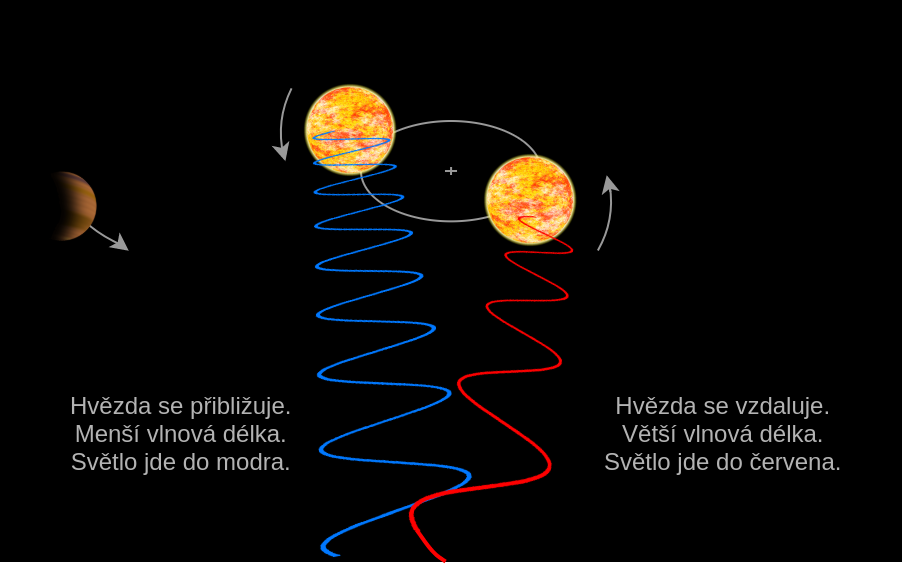
\includegraphics[width=\textwidth]{img/radial_velocity.png}
\caption[Metoda radiálních vzdáleností]{Metoda radiálních vzdáleností \footnotemark[1]}
\end{center}
\end{figure}

\footnotetext[1]{Vytvořeno autorem v \url{https://www.draw.io} a GIMP.}


%%%%%%%%%%%%%%%%%%%%%%%%%%%%%%%%%%%%%%%%%%%%%%%%%%%%%%%%%%%%
% POUŽITÁ LITERATURA
%%%%%%%%%%%%%%%%%%%%%%%%%%%%%%%%%%%%%%%%%%%%%%%%%%%%%%%%%%%%

\clearpage \phantomsection \addcontentsline{toc}{section}{\refname}

\begin{thebibliography}{99}	% parametr určuje nejširší položku

% nezlomitelné spojovníky lze zapisovat zkratkou "- nebo příkazem \babelhyphen{nobreak}

\bibitem{methods}
Metody objevování planet.
\textit{Astronomia.} [online]. 23.~1.~2013. [cit.\,23.~12.~2019].
Dostupné z: {\ttfamily \url{http://hvezdy.astro.cz/exoplanety/51-metody-objevovani-planet}}.

\end{thebibliography}

%%%%%%%%%%%%%%%%%%%%%%%%%%%%%%%%%%%%%%%%%%%%%%%%%%%%%%%%%%%%
% KONEC DOKUMENTU
%%%%%%%%%%%%%%%%%%%%%%%%%%%%%%%%%%%%%%%%%%%%%%%%%%%%%%%%%%%%

\end{document}